% !TeX root = ../Thesis.tex
\chapter{Proof of Latency}
\label{Proof of Latency}
Proof of Latency, "the algorithm" or "PoL", is a collection of two algorithms that when used in a P2P context, can offer a robust way of reducing network latency between peers on the network by minimizing the number of hops between peers that are close in terms of performance and geographical location.

The first version of the algorithm requires a trusted setting, preferably a trusted computing platform from all participating peers, while the second version is trustless and requires no specific hardware from the participants, while a trusted computing platform would make it fairer and more reliable, by not discriminating based on CPU performance. An ASIC VDF chip would also mitigate any of the later mentioned attack vectors by removing variance in hardware.

\section{Role of Latency in Distributed Systems}
It's hardly a surprise, but latency is a huge factor in distributed systems, especially trustless, decentralized ones. Latency is mostly constrained by the speed of light, which can not be changed, and thus there are concrete factors that must be taken into account when designing a p2p system with routing. In 2012, the global average round-trip delay time to Google's servers was around 100ms.\cite{Grigorik_undated-mc}

In the new space age the maximum possible latency grows very fast, as there could be peers joining to a distributed network from other planets, space ships or stations. This might be unnecessary to think about in the distributed P2P context for now, but before all that, we have global satellite mesh internet providers, like Starlink. Elon Musk, the founder of SpaceX, which provides the network of satellites, claims that there's going to be a latency of about 20 milliseconds.\cite{Tung_undated-ny} But, since speed of light restricts us to about 100ms of minimum global latency, those claims cannot be trusted. In legacy satellite internet access, the round-trip time even in perfect conditions is about 550 milliseconds.\cite{noauthor_undated-zc}

\section{Network Hops Increase Latency}
Network hops in P2P systems are introduced when two peers are not directly connected to each other, but rather through one or many relays. There are network hops that cannot be easily avoided, like the hops between network routers in the internet already. Most of the P2P routing protocols used today are oblivious to the problem of introducing large hops to communications between two peers. These DHT-based protocols, like Kademlia, make the assumption that their users have fast internet access, and minimize the average latency by selecting connected peers basically at random.

While the randomness is great for preventing eclipse attacks, they can introduce unnecessary geographical hops between two peers. If two peers are in the same WAN, for example, in Kademlia they might still connect to each other through a network hop going through another continent. This makes individual connections less efficient.
Now, if we were to rely on IP address geolocation, we could more efficiently connect to peers that are close-by. This is unfortunately impossible in privacy-oriented P2P networks, like mixnets, which aim to hide as much of the packet routing information as possible, by routing individual packets through different peers and hiding IP addresses of two connected peers from each other.\cite{Harry_Halpin_undated-sq}

Proof of Latency is made to improve the performance of current P2P networking solutions and make them future-proof, even for hops between planets, while still being compatible with some privacy-preserving P2P protocols, since it is agnostic of the addressing method used.

\section{First Version of PoL}
The first iteration of the algorithm is based on an attempt to simplify the initial Proof of Latency algorithm. After some thought, I came to the conclusion that the initial iteration, which ended up as the second and final version of the algorithm, is actually the most resistant to attacks and requires less trust from the participants.
\begin{figure}
	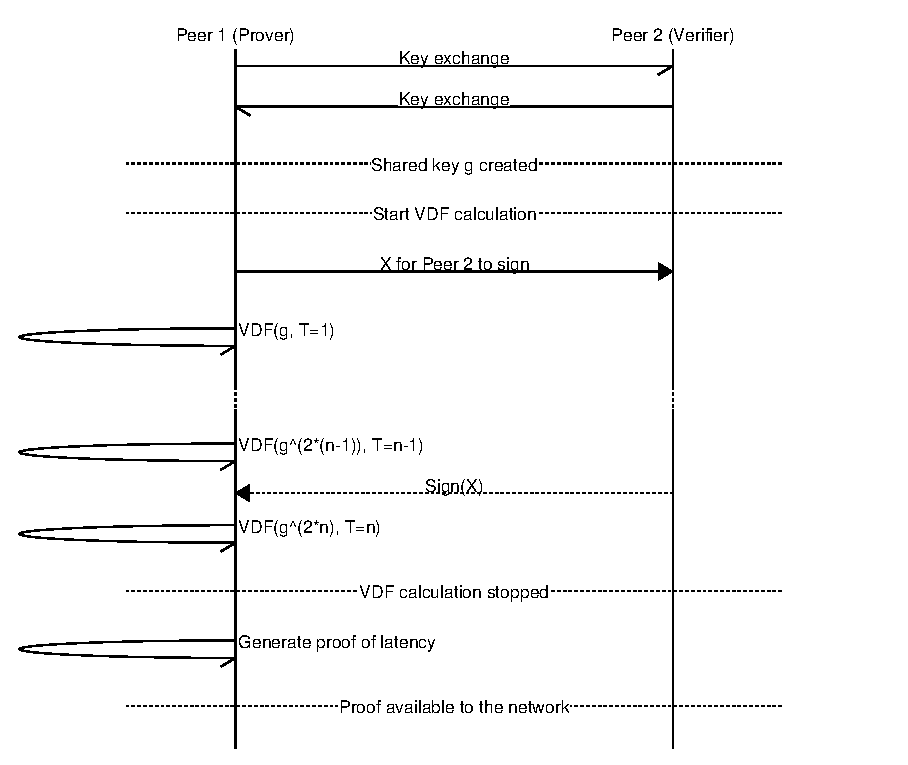
\includegraphics[width=\textwidth]{pictures/pol1_diagram.eps}
	\caption{Proof of Latency, Version 1}
	\label{PoL Diagram 1}
\end{figure}

\subsection{Results}
Since the network peers are trying to compete with each other for the least latency, they win the game by calculating the least amount of VDF iterations. In the first version of the algorithm, this soon becomes a problem. There's no way to tell how fast another computer is, so in this case spoofed results of 1 iteration would win every time.

This version only works if the peers can trust each other, but in that case we could also resort to using ping. Ways of introducing trust would be using a trusted computing platform, but even that could be vulnerable to undervolting or other physical tampering. This problem drove me to revert back to my original idea, which I'm calling the version two of Proof of Latency.

\section{Second Version of PoL}
\begin{figure}
	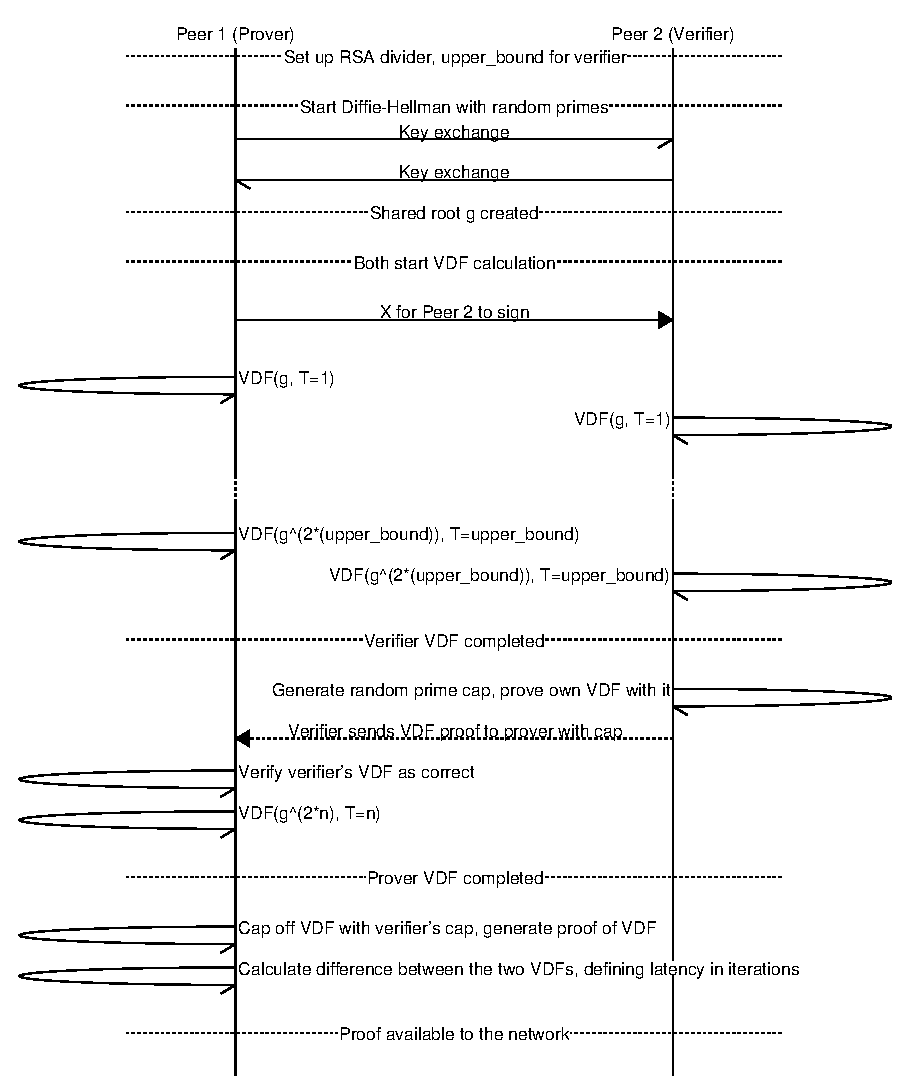
\includegraphics[width=\textwidth]{pictures/pol2_diagram.eps}
	\caption{Proof of Latency, Version 2}
	\label{PoL Diagram 2}
\end{figure}
The second version of PoL introduces a race between the two peers. Like in the first version, there's a prover and a verifier. The difference here is that they both calculate a VDF and the verifier calculates the difference in iterations between the two.

First the prover and the verifier do a Diffie-Hellman key exchange to construct a previously unknown key. Then, they both start calculating a VDF in parallel. The prover only calculates the VDF up to a predefined threshold, and then sends the proof with a signature back to the verifier. The verifier then stops its own calculation, generates a proof of it, and then calculates the absolute difference between the amount of iterations between its own VDF and the prover's.

Since calculating a VDF is relatively easy for modern processors, a VDF over as little as a few milliseconds of time can be a valid way of measuring latency. Still, without an ASIC chip for calculating VDFs faster than any other available processor, these protocols are also a measurement of processing performance. This might introduce an unfortunate barrier for entry for mobile and IoT devices. The second version of PoL is meant to tackle this problem by creating a performance and latency gradient to the network. The network topology results in a gradient that is defined by geographical location and the similarity in performance. This means that connectedness between mobile and IoT devices is going to be better than between devices that have a huge performance difference.

\section{Attack Vectors}
Since Proof of Latency removes security quarantees by removing randomness from routing, some new attack vectors are introduced. The two versions of the algorithm differ much in terms of security.

\subsection{Performance Matching}
Both versions suffer from the same issue, let's call it performance matching, which is a timing attack. Timing attacks are a family of attacks against computer systems called side-channel attacks, which attack the fact that although software is abstract and can be very well fit against any attacks on the software level, outer factors still affect the hardware it runs on. Timing attacks rely on gathering of timing data from the target.\cite{noauthor_undated-mp} In performance matching, this means connecting to the targeted peer by another protocol or comparing existing proofs of latencies from all peers that have calculated their latency with the target.

Performance matching enables attackers to perform an eclipse attack on low-performance devices by matching the attacker's performance with the targeted mobile device so that it is as close as possible in the difference between iterations in PoL. Now again, if the algorithm had a trusted platform module requirement, or we had an ASIC for repeated squarings, this wouldn't be an issue on either of the versions of the algorithm. This attack could result in a complete network split.

\section{Protecting Against Performance Matching}
\subsection{Zero-Knowledge Proofs}
Zero-knowledge proofs could be used to protect against performance matching. If the publicized proof didn't include both the VDF results and iterations, but just included the iteration difference, an attacker would have less info on each peer. This would make attacking more difficult, requiring more queries and PoL runs on average before finding a vulnerable peer.

\subsection{Web of Trust}
There's also a possibility of introducing a web of trust in parallel to PoL to recognize and shut out malicious peers more effectively. An example of such a system is SybilLimit, which adds a construction called trusted routes to DHT-based routing.\cite{Yu2008-xl}

\subsection{Switch Responsibilities}
This remedy aims to improve PoL version 1 by flipping the responsibilities of the prover and the verifier. The calculating party wants to prove its latency to the verifier by actually calculating the VDF itself, requiring the verifier to respond as fast as it can to the prover's messages. This way, only a proof of one VDF is needed, which the prover then advertises to the network, telling connecting peers exatly the number of calculations it got to calculate before the verifier responded to it. 

There's a catch, though. The prover can still lie to other peers by slowing down their VDF calculation. By flipping the responsibilities the protocol becomes trustless for the prover, but not for others. The flip felt promising at first glance, but I soon realized there's no better way to do this than the second version, where trust is shared and not assumed.

\chapter{Proof of Concept}
\label{Proof of Concept}
To test out Proof of Latency, I made a software proof of concept in Rust, using some open source projects, blog posts and previous knowledge as a base for the work. 
